%!TEX root = ../../secondYearReport.tex
\paragraph{Work package 2 progress}


\subparagraph{Design of models for human whole body motion in contact (T2.2)}
In the scope of T2.2, JSI created a 3D dynamic model of a human holding to a stable object during continuous perturbations of stance. The model was devised from measurements on 13 male subjects. Using the kinematical data recorded with frequency of 100Hz, forces that the subjects excerted on the ground, and the forces in the handle, we performed an inverse dynamic procedure and obtained joint torques produced by muscles during the experiment. An illustration of the model is shown in Fig. \ref{fig:skeleton}. Using this modelling approach we are now able to efficiently study the biomechanics of humans in contact with the environment.

\begin{figure}[!t]
	\begin{center}
		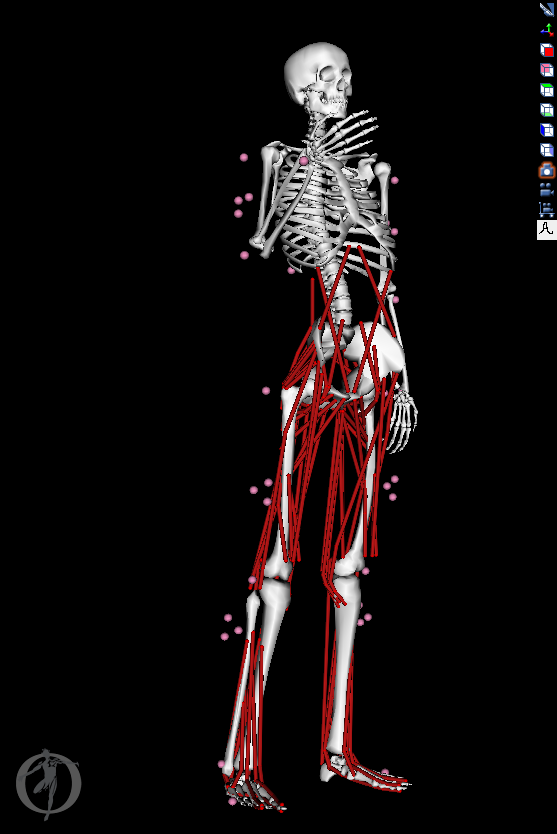
\includegraphics[width=0.5\textwidth]{skeleton_v1.png}
		\caption{Model of a subject holding a handle.}
		\label{fig:skeleton}
	\end{center}
\end{figure}


During the second year of the project, UB studied the effects of hand contact
on the stability of a planar humanoid robot (see Fig.~\ref{planarhumanoid})
while a momentum based controller is used to control the robot's balancing
motion \cite{Azad2014}. They compared the simulation results with the
results of the experiments on human subjects which are reported in
\cite{Babic2014}. Both simulations and experiments agreed that different
values of hand contact forces in different hand positions cause the same
displacements of the CoP of the foot. This implies that regulating the CoP of
the foot has the highest priority for both humans and the momentum based
controller.  This study suggested that the momentum based controller is an
adequate controller to replicate human behaviour during balancing motions.

\begin{figure}[!t]
  \centering
	\begin{subfigure}[b]{0.45\textwidth}
	\centering
  	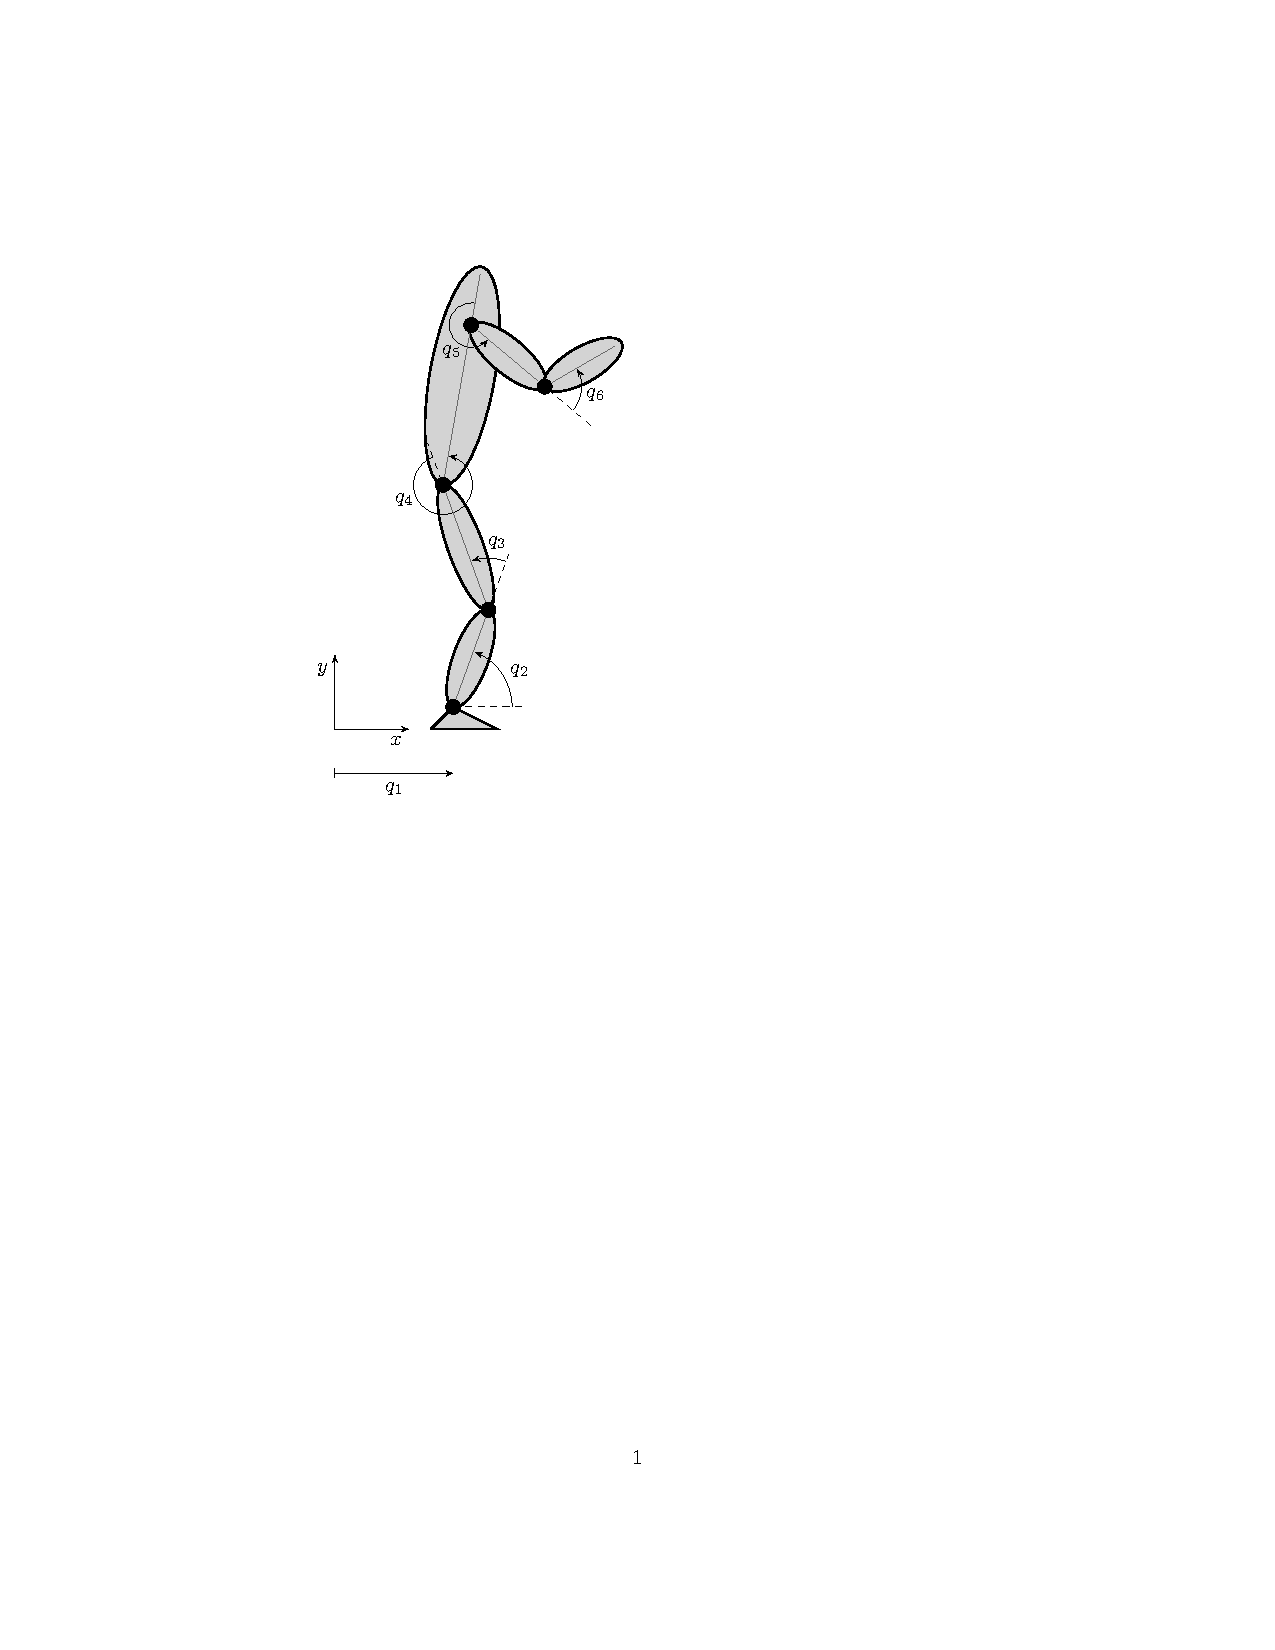
\includegraphics[trim=53mm 144mm 110mm 44mm, clip,
    scale=0.8]{planarhumanoid.pdf}
	\subcaption{Schematic diagram of the robot model and its coordinates}
   \label{planarhumanoid}
	\end{subfigure}
	\begin{subfigure}[b]{0.45\textwidth}
	\centering
	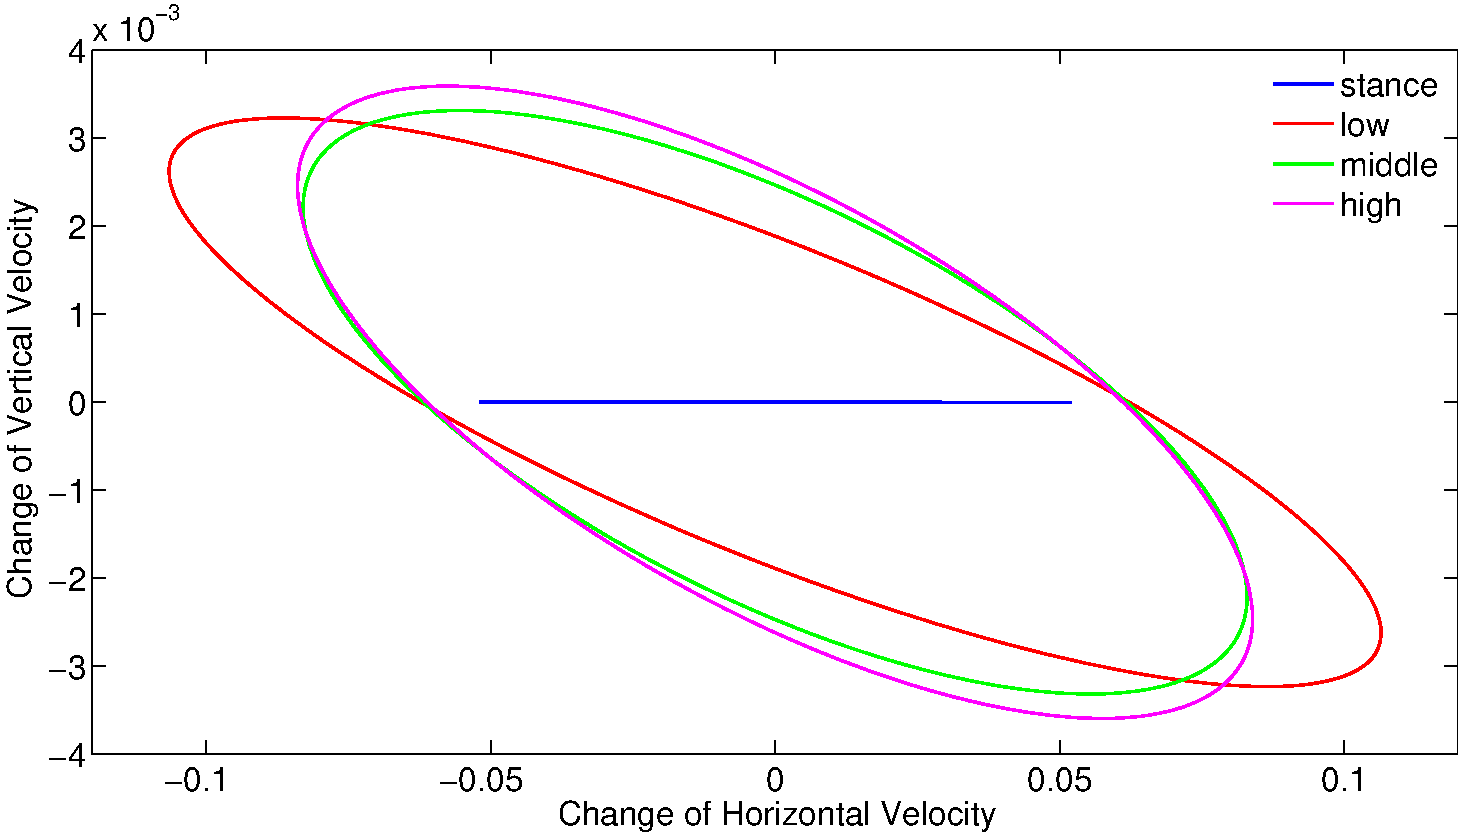
\includegraphics[trim=45mm 0mm 65mm 5mm, clip, scale=0.5]{ellipses.pdf}
	\caption{Velocity ellipses for a planar humanoid robot}
	\label{ellipses}
	\end{subfigure}
\end{figure}

During the second year, UB continued to work on defining a suitable metric to
measure the effects of the environmental contacts on the robot's stability.
They used the basic concept of end-effector manipulability (for manipulators)
in the literature and introduced a new tool to analyze the ability of balance
for legged robots which we called it manipulability of the center of mass.
This tool defines three different types of ellipsoids which are called 1)
velocity ellipsoid, 2) instantaneous velocity ellipsoid and 3) instantaneous
velocity ellipsoid due to the unit impulse.  The first one shows the velocity
of the CoM in different directions due to the unit norm of the joint
velocities.  The second and third types of the ellipsoids, which are obtained
by using impulsive dynamics, show instantaneous changes of the CoM velocity
due to the unit norm of instantaneous changes at the joint velocities and the
unit norm of impulse at the actuated joints, respectively.  By involving the
motion equations into the calculations for the second and third types of
ellipsoids (via impulsive dynamics), these ellipsoids allow us to study the
effect of under-actuation as well as kinematic constraints on the robot's
stability.

As an example, Fig.~\ref{ellipses} shows a planar humanoid robot (with its hand 
is fixed) and instantaneous velocity ellipses for the robot in the
specified configuration. Since the robot is fully actuated, the first and
second types of ellipses (type 2 and type 3) are the same. This ellipse (type
2) shows how the velocity of the CoM changes when the instantaneous change of
the joint velocities due to the impulse has the unit norm. This shows the
ability to move the CoM in different directions by a certain amount of
movements at the actuated joints. The ellipse type 3 shows how the velocity
of the CoM changes due to the unit impulse at the joints. In other words, it
shows how a certain amount of impulse at the actuated joints can accelerate
the CoM in different directions. All of the ellipses are independent from the
controller and they are dependent only on the physical parameters of the robot
and its kinematic constraints.

In balancing in a plane, the CoM movement in the horizontal direction is an
important measure. By projecting a velocity ellipse on $x$ axis, we obtain a
line which its length equals to the maximum change of velocity of the CoM in
the horizontal direction. Figure \ref{type2} (left side) shows maximum
instantaneous change of the CoM velocity in the horizontal direction for
different constrained hand locations (i.e. different elbow and shoulder
angles). This is due to the unit norm of instantaneous change of the joint
velocities. In the right side of this figure, the graph at the left side is
compared with the case that the hand is not constrained. It is obvious that
the movement of the CoM is limited due to the kinematic constraint at the
hand.
\begin{figure}[!t]
  \centering
  \begin{tabular}{lr}
    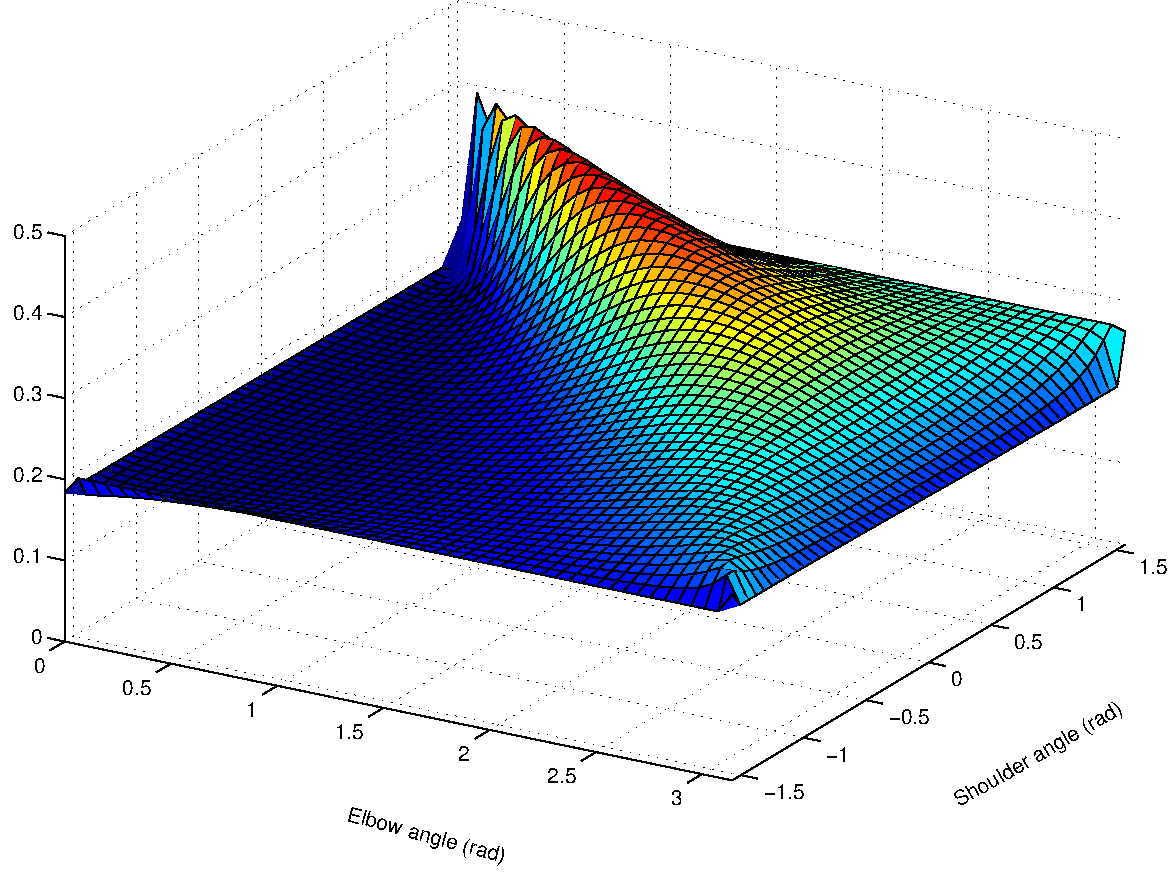
\includegraphics[scale=0.38]{type2_2.pdf}
    &  
    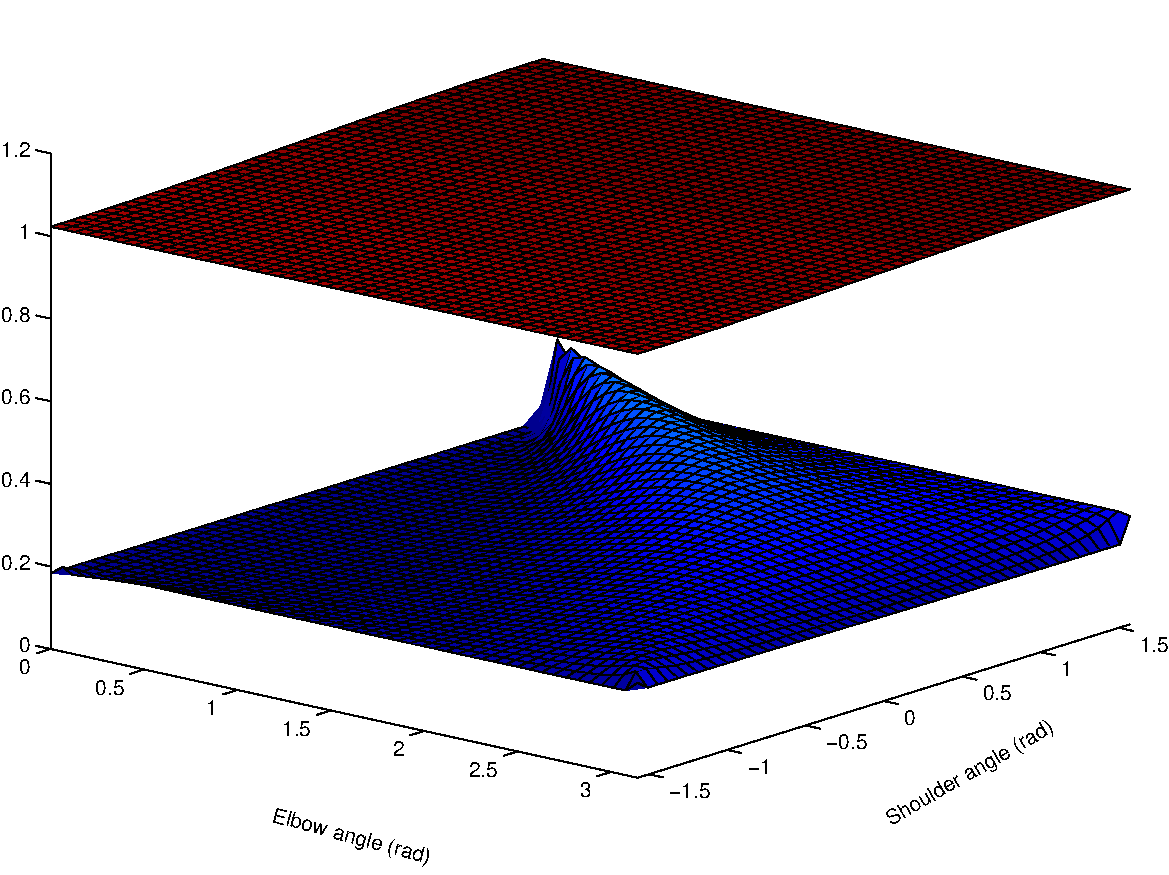
\includegraphics[scale=0.38]{type2.pdf}
  \end{tabular}
  \caption{Maximum instantaneous change of the CoM velocity in the $x$
    direction due to the unit norm of instantaneous change of the joint
    velocities for (left) the constrained robot and (right) for both
    constrained and unconstrained robots.}
  \label{type2}
\end{figure}

Figure \ref{type3} shows maximum instantaneous change of the CoM velocity due
to the unit impulse at the joints for different hand locations and for both
constrained and unconstrained hands. As it can be seen in this figure, the
graph for the constrained robot is always higher than the other one. This
implies that the same amount of impulse can cause bigger changes at the CoM
velocity in the constrained robot rather than the unconstrained one. The
reason is that, in the constrained case, the robot exploits the contact force
to accelerate the CoM and therefore less (impulse) torque is needed for the
same change at the CoM velocity.
\begin{figure}[!t]
  \centering
  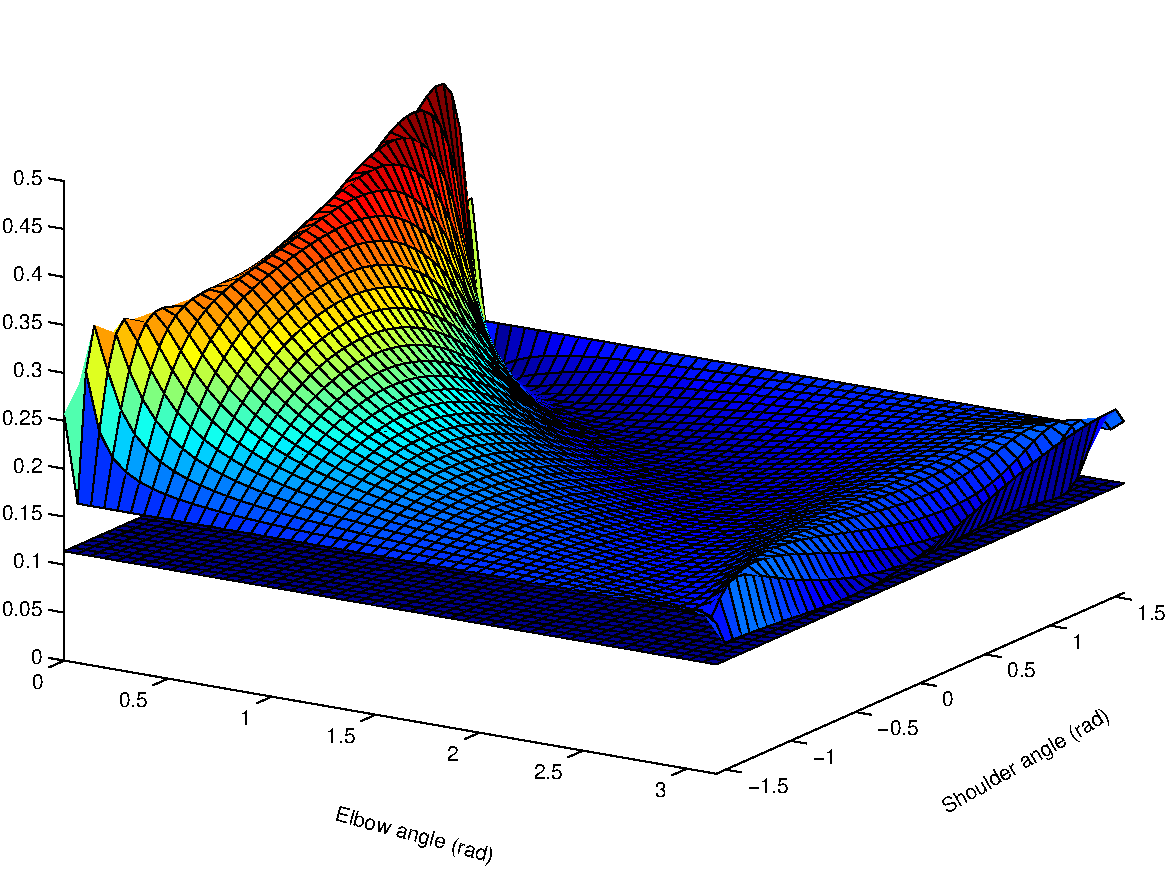
\includegraphics[scale=0.5]{type3.pdf}
  \caption{Maximum instantaneous change of the CoM velocity in $x$ direction
    for the constrained and unconstrained robots due to the unit norm of
    impulse at the joints.}
  \label{type3}
\end{figure}







\subparagraph{Strategies of dealing with uncertainties in contact (T2.3)}

During the second year work on T2.3, JSI developed a novel method to study human strategies of dealing with contacts with uncertain environment. In this method the human subject was made to perform psychical contacts with the environment through the robot. The human was included into the robot control loop through human-robot interfaces. The idea is that the human sensorimotor system and cognitive system controls a novel mechanical system, i.e. the robot, in physical interaction with the environment. This implies additional human motor control learning and adaptation that can potentially provide us with a deeper insight into how humans deal with a novel environment.

Another advantage of this approach is that the human sensorimotor system does not use its own limbs to directly make the contacts with the environment, but uses the robotic limb to do so. Compared to pure biomechanical studies, where the measured human behaviour must be further interpreted, adjusted or transformed before it can be used on the robots, in this approach the measured human behaviour can be directly captured and used in the robot control. This study therefore provides a good complement to our conventional biomechanical studies as performed in T2.2.

The block scheme of the proposed approach is shown in Fig. \ref{fig:scheme}. The human controlled the motion of the robotic limb with the motion of his/her own limb. In addition to controlling the motion, the human also controlled the impedance of the robot. Primary information about the robot state was relayed to the human through a visual feedback. A haptic device was used to provide the human with an additional feedback about the forces sensed by the robot. While controlling the robot in the proposed human-in-the-loop approach, the human central nervous system had to adapt to a new mechanism through sensorimotor learning to perform the desired contact with the environment.
\begin{figure}[!t]
  \centering
  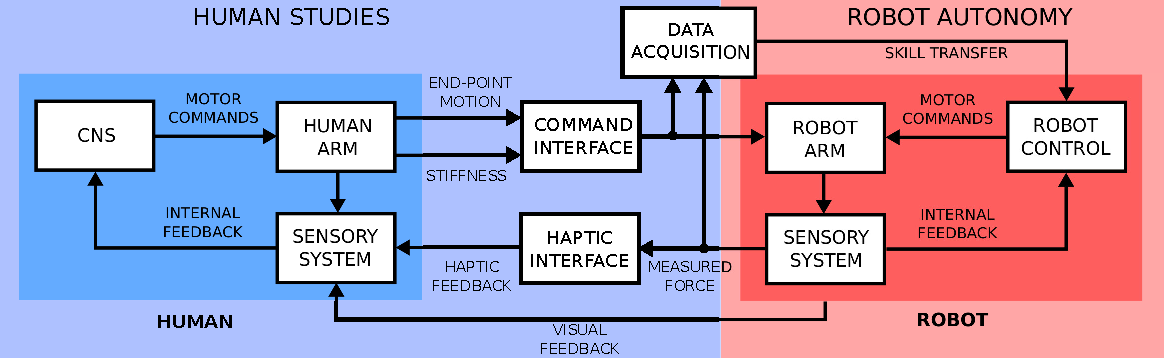
\includegraphics[width=0.9\textwidth]{scheme.pdf}
  \caption{Block diagram of proposed human-in-the-loop robot control framework for study of human behaviour in contacts with environment. During the learning and adaptation stage, the human performs the contacts with the environment through the robot (blue section). The acquired data was used to observe and study the human behaviour. When the human learning process and observation is complete, the learnt skill can be directly captured and used in the autonomous robot control (red section). This is the main advantage compared to the conventional biomechanical studies.}
  \label{fig:scheme}
\end{figure}

The main goal of studies of human behaviour in contacts with environment in WP2 is to offer a basis from which we can devise equivalent humanoid robot behaviour. The most appealing prospect of the proposed approach to study human motion in contacts with the environment is that the data from the study can be used to directly form skills for autonomous robot control. The sensorimotor data was collected while the human was making the desired physical contacts with the environment though robotic mechanism. This data was then used to form the trajectories. The trajectories were encoded with Dynamical Movement Primitives (DMPs) \cite{Ijspeert2002}. The parameters of DMPs were learned by locally weighted regression \cite{Schaal1998}. The learned trajectories represented the robot skill for dealing with the contacts with the environment according to the human strategy. The trajectories can be included into the robot control system and used for autonomous execution of the learnt task.
\begin{figure}[!t]
\centering
\begin{subfigure}[b]{0.43\textwidth}
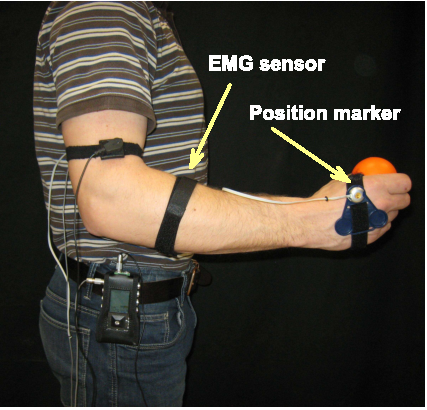
\includegraphics[width=1\textwidth]{emg_setup.pdf}
\end{subfigure}
\begin{subfigure}[b]{0.53\textwidth}
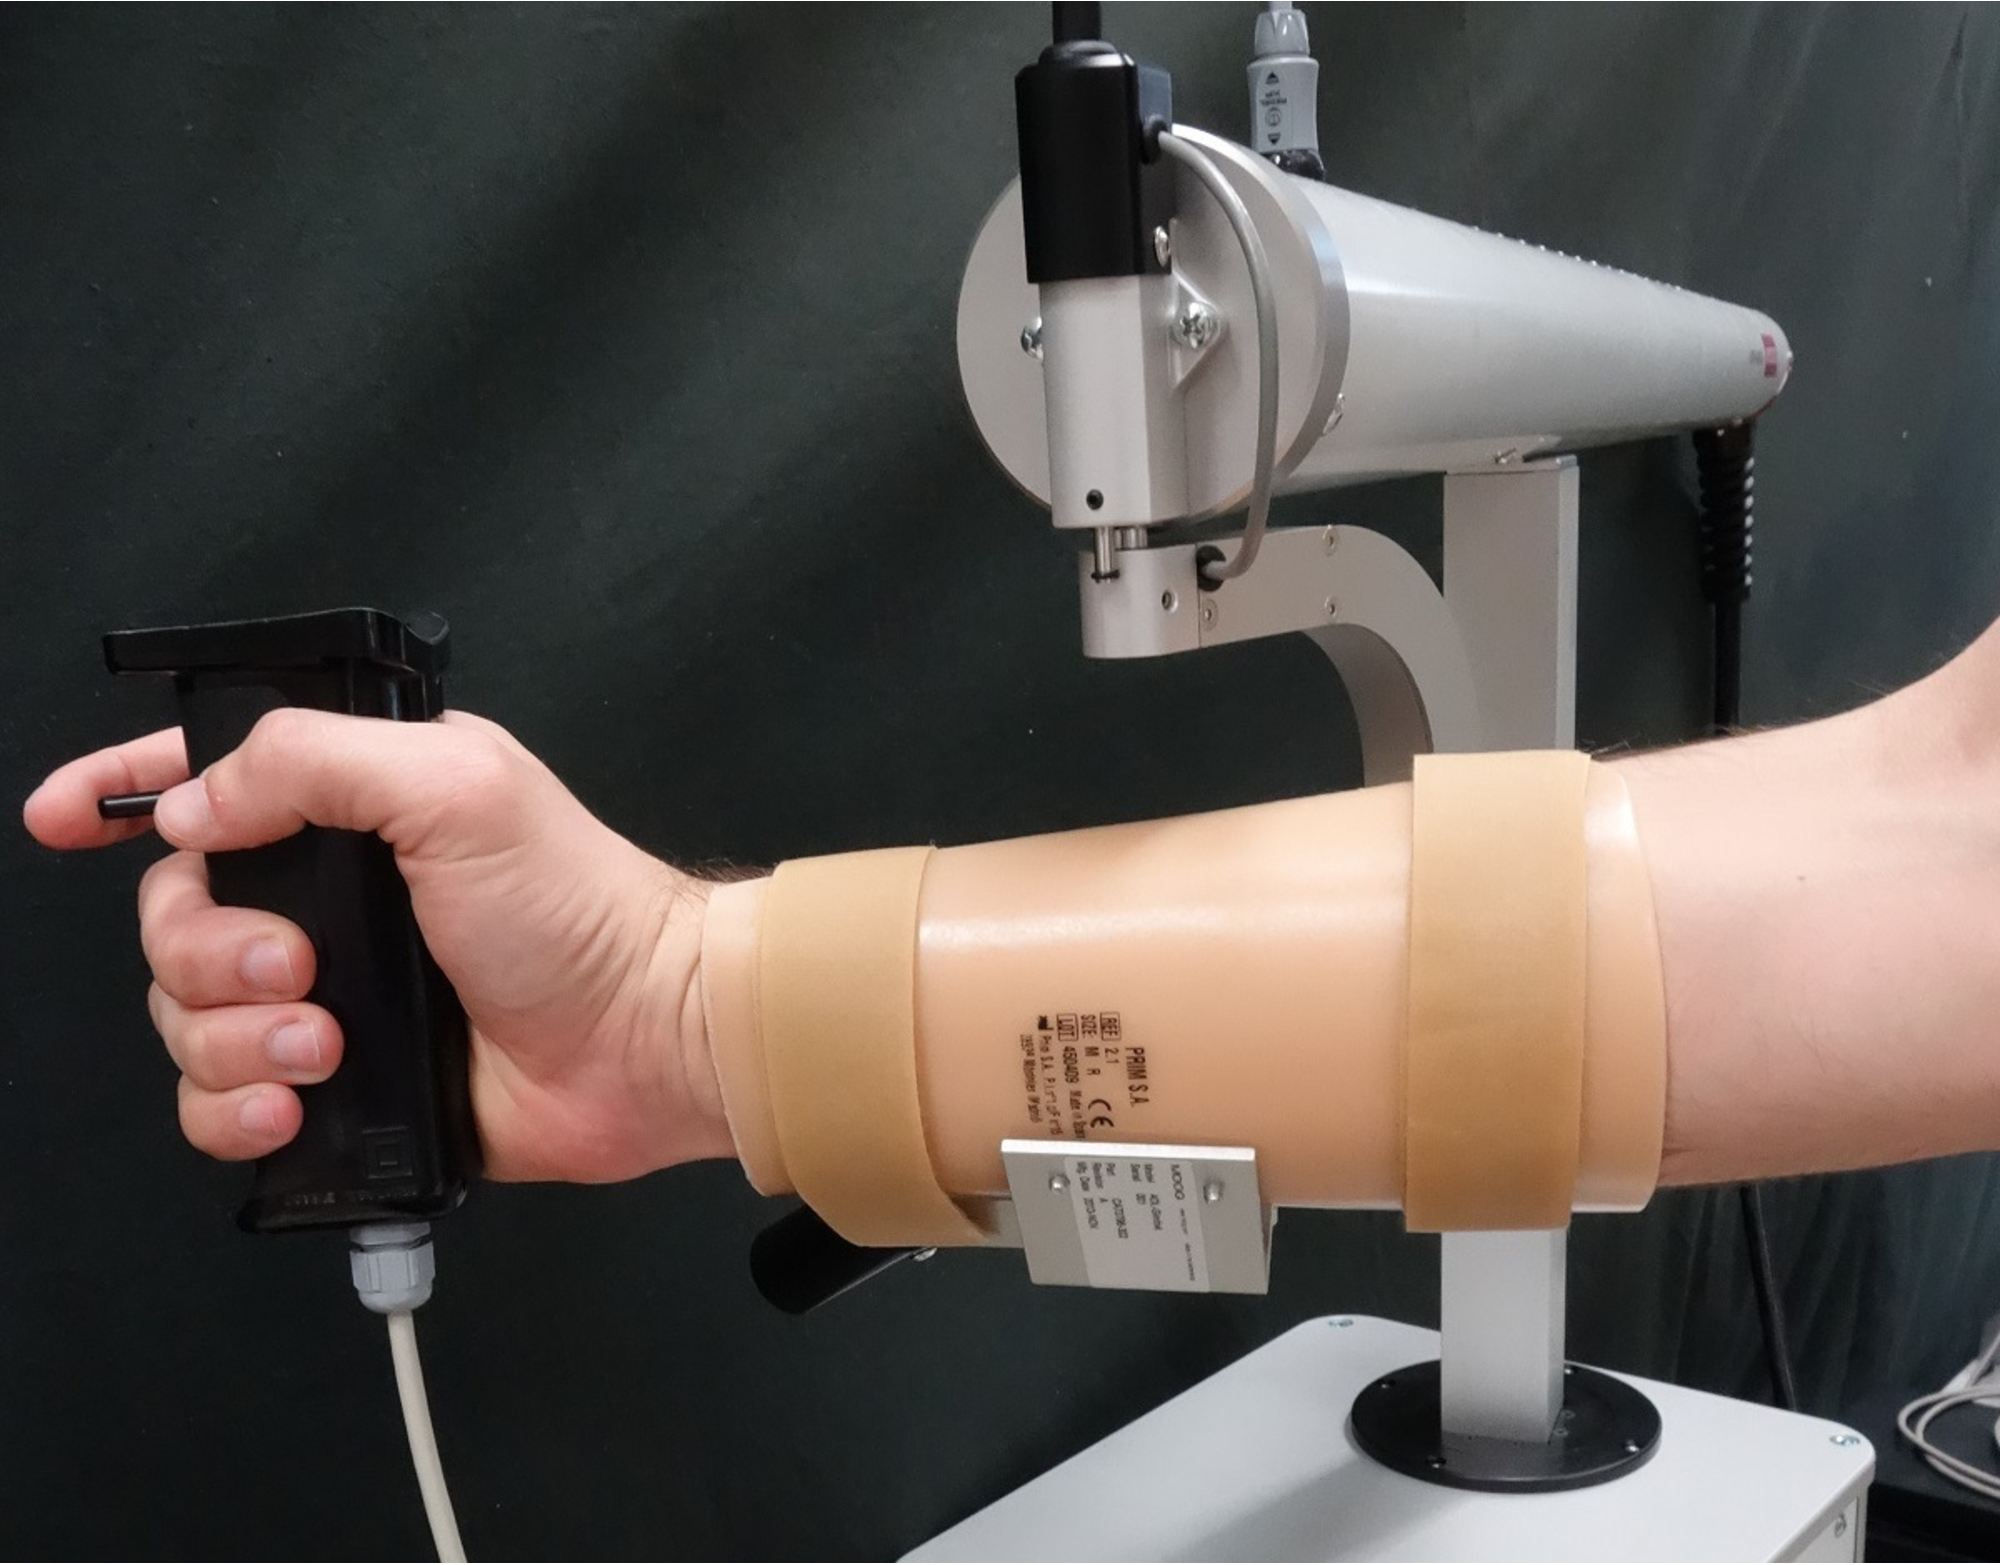
\includegraphics[width=1\textwidth]{haptic.pdf}
\end{subfigure}
\caption{Human-robot interfaces. First developed interface (left) measured human limb motion via optical motion capture system and mapped it to the motion of the robotic limb. The human muscle activity was measured by sEMG and was used as an interface to control the robot impedance. Second developed interface (right) consisted of \textit{HapticMaster} robot and impedance control handle. \textit{HapticMaster} robot measured the human limb position and provided the force feedback. Impedance control handle was based around a spring-return linear potentiometer and was held in the human hand.}
\label{fig:interface}
\end{figure}

One of the key features of the proposed approach is the ability of the human to directly control the impedance of the robot limb in an equivalent way that he/she controls his/her own. For this purpose we developed two novel human-robot interfaces \cite{Peternel2014,Peternel2015} that allow the human to modulate the stiffness of the robotic limb in real-time. The first interface (see Fig. \ref{fig:interface}, left) was based on measuring human muscle activity by surface electromiography (sEMG). The current measured muscle activity was mapped to the robot stiffness. The second interface (see Fig. \ref{fig:interface}, right) was based around a linear potentiometer inside a handle held in the human hand. The human controlled the position of the potentiometer knob with a finger position. The finger position is then mapped to the robot stiffness via measured potentiometer voltage.








\subparagraph{Human contact choice and learning through physical interaction (T2.4)}

Within T2.4, Inria, TUD and UPMC participated in analysing the dataset of the EDHHI experiments\footnote{\url{http://www.loria.fr/~sivaldi/edhhi.htm}} where healthy adults (18-65 years old) interact physically with the iCub (see  Fig.~\ref{fig:eddhi_picture}). The analysed data include tactile data from the forearm skin and contact forces, estimated by the iDyn modules developed in WP1. The preliminary analysis shows that people, on average, learn quickly how to interact with the robot and move its arms: across three trials, the exchanged forces are smaller and the contacts more precise. Currently, Inria is coupling the analysis of tactile and force signals with individual factors and social signals exchanged by the two peers.

\begin{figure}[!t]
  \centering
  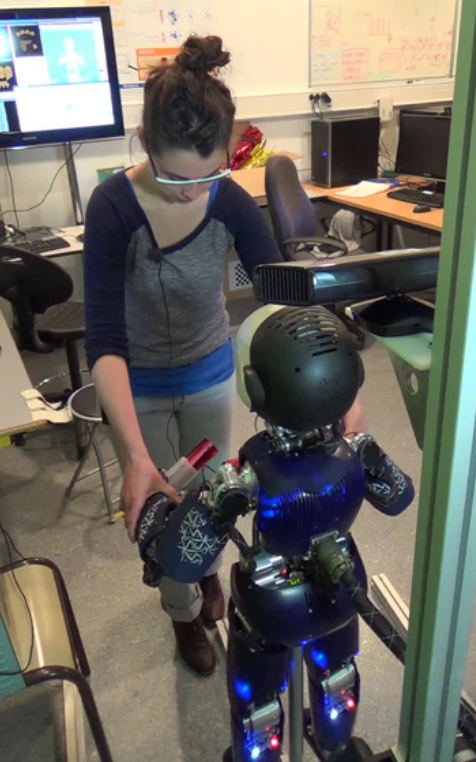
\includegraphics[width=0.48\textwidth]{eddhi_illustration.png}
  \caption{View of a physical interaction between a human and the iCub robot.}
  \label{fig:eddhi_picture}
\end{figure}

In the scope of T2.4, JSI studied how additional hand contact with the surrounding objects influences whole-body balance conditions. The experiments were performed on multiple subjects where we challenged their balance. The experiments were divided into two main stages. Each stage had 15 sessions in which the subject's balance was perturbed for 5 minutes. In one stage the subjects did not use supportive hand contact. In the other stage they were holding a handle in front of them. We used a motorised wait-pull mechanism \cite{Peternel2013} to continuously perturb the balance of the standing subjects in either stage by exerting external forces on the approximate position of centre of mass. See Fig. \ref{fig:exp2_protocol} for the experimental setup.

\begin{figure}[!t]
	\begin{center}
		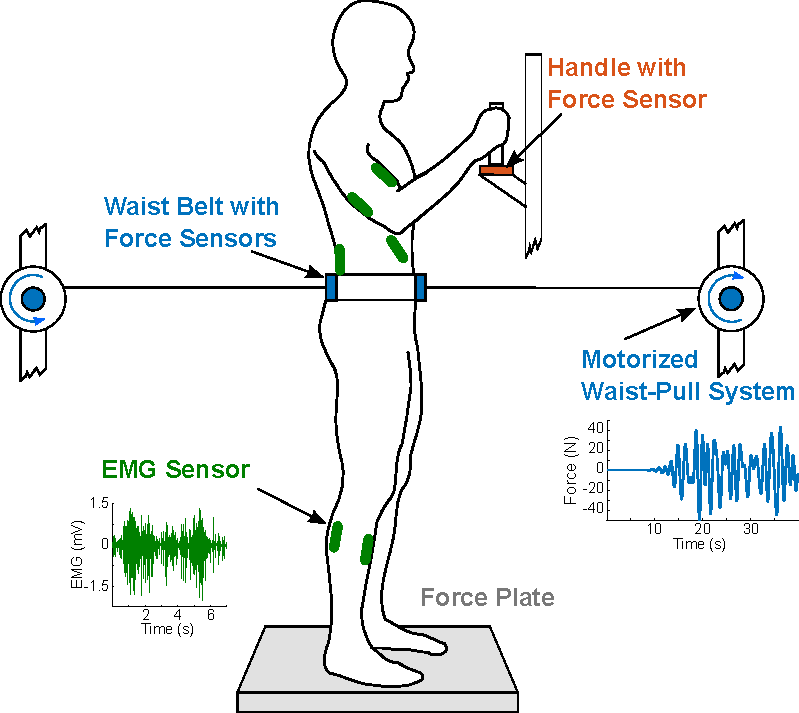
\includegraphics{exp2_protocol.pdf}
		\caption{The subject was standing on a force plate, connected to the motorised waist-pull system that generated translational perturbations. The subject was holding the handle with a built-in force sensor mounted on a vertical pole. EMG electrodes were positioned on the major body muscles of the subject's right-hand side.}
		\label{fig:exp2_protocol}
	\end{center}
\end{figure}

The perturbation waveform of the waist-pull mechanism was constructed in a way that the possible muscle reactions associated with reflexes were eliminated. These reactions could potentially mask the actual role of the hand muscles as the reflex would activate the muscles unrelated to the magnitude of the perturbation. To avoid that, the perturbation waveform was continuous, had relatively low frequency and low pulling forces. During the experiment, we measured muscle activation of the subject's lower leg, trunk and arm muscles, forces in the handle and the anteroposterior movement of CoP (CoP$_{AP}$).

The results of muscle activation analysis showed that when the subjects were holding to the handle, the activation of the leg muscles was minimal (see Fig. \ref{fig:representativePSD}). Based on this we can conclude that the subjects mainly used their arm muscles to maintain postural stability. The trunk flexor muscle (Obliques Externus, OE) was more active in the stage when the subjects were holding the handle compared to when they were not. This indicates that a synergy between the arm and trunk muscles was established when additional hand contact was utilised to maintain the equilibrium.

\begin{figure}[!t]
	\begin{center}
		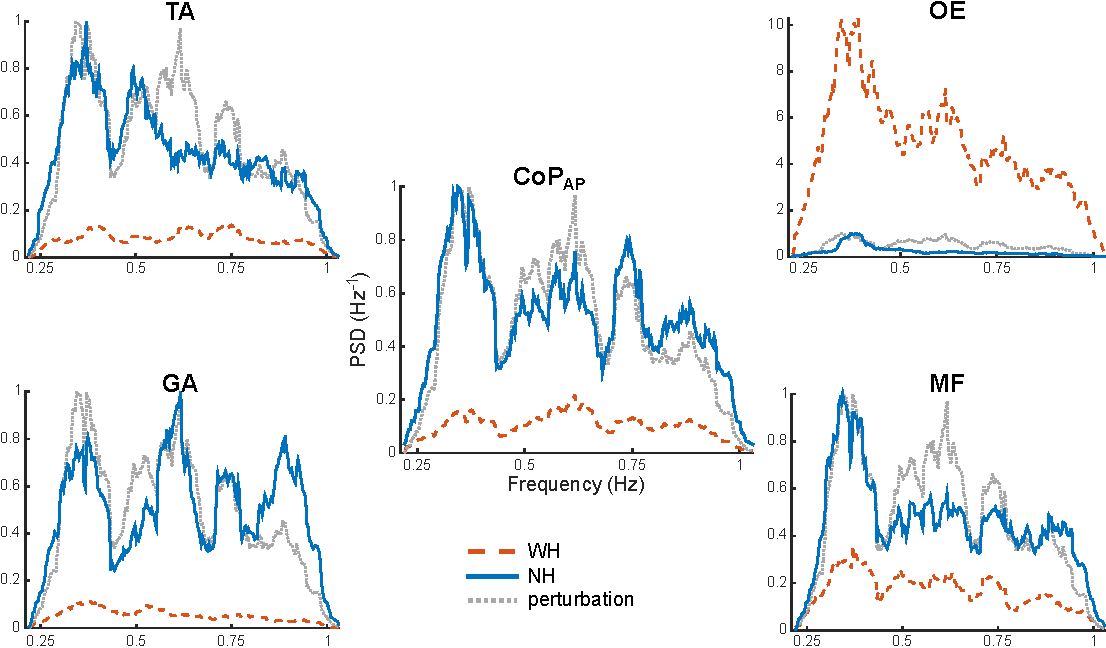
\includegraphics[width=\textwidth]{representativePSD_oneYaxis-v1.pdf}
		\caption{Effect of holding a handle after adaptation stabilised in the last session. The graphs show representative power spectral density (PSD) profiles of CoP$_{AP}$ and muscle activations measured in trunk and lower leg muscles. After the adaptation, effect of additional supportive hand contact stabilised to the perturbation in the last session. All EMG and CoP$_{AP}$ values are presented in a frequency domain, ranging from 0.25 Hz - 1 Hz. The blue (solid) lines represent the power in no-handle and the orange (dashed) lines in handle stage. The grey (dotted) line is the power of the perturbation signal. All signals are normalized to the peak value in the last session. The effect of handle is shown as reduced muscle activation in all muscles in the handle session, except in the trunk flexor muscle (OE), where there is an opposite effect.}
		\label{fig:representativePSD}
	\end{center}
\end{figure}

The analysis of the CoP$_{AP}$ movement showed that the displacement of the CoP$_{AP}$ was progressively dropping throughout the repeated sessions of the experiment (see Fig. \ref{fig:COPapAndTau}). This was true both in case when supportive hand contact was used and in case when no supportive hand contact was used. These results give a strong hint that a learning and adaptation was present through the sessions of the experiment, as the subject gradually improved the balance control.

\begin{figure}[!t]
	\begin{center}
		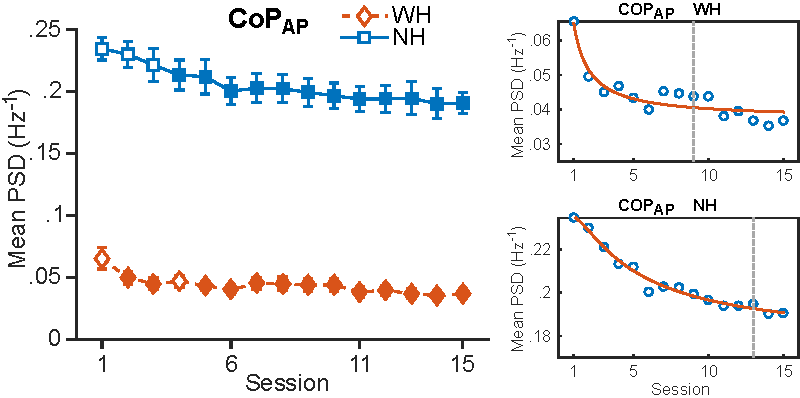
\includegraphics[width=\textwidth]{COPapAndTau.pdf}
		\caption{Adaptation of movement of CoP$_{AP}$ is shown on the left graph. Experimental stage with handle (WH) is shown in red, while condition without handle (NH) is shown in blue. Full markers indicate statistically significant differences between the first session and each of the following sessions. In both stages the adaptation is statistically confirmed (\textit{p} < .001). In the stage where the subjects were holding the handle, the adaptation appeared right after the first session. In no-holding stage it appeared after the third session. The superimposed best-fit curves are shown on the right graphs with orange solid lines. A calculated session number at 3$\tau$ of the fitted curve (vertical dotted line) indicates faster stabilisation of adaptation in the handle stage, compared to no-handle stage.}
		\label{fig:COPapAndTau}
	\end{center}
\end{figure}

We further analysed whether there are any effects of repeated sessions on adaptation of muscle activation and movement of CoP$_{AP}$ (Figure \ref{fig:meanErrorBars}), and whether there are any differences between the two stages of the experiment. The results show that the effect of human adaptation in lower leg muscles was statistically significant in the stage when the subjects were not using the additional hand support. However, this was not the case for the stage when the subjects were holding to the handle.

The activation of the trunk extensor muscle (MF) was almost the same in both stages and throughout all sessions. On the other hand, the activation of the trunk flexor OE remained unchanged throughout the sessions only in the stage when subjects held the handle. The activation of OE was much higher in this stage compared to stage when subject did not use supportive hand contact.

\begin{figure}[!t]
	\begin{center}
		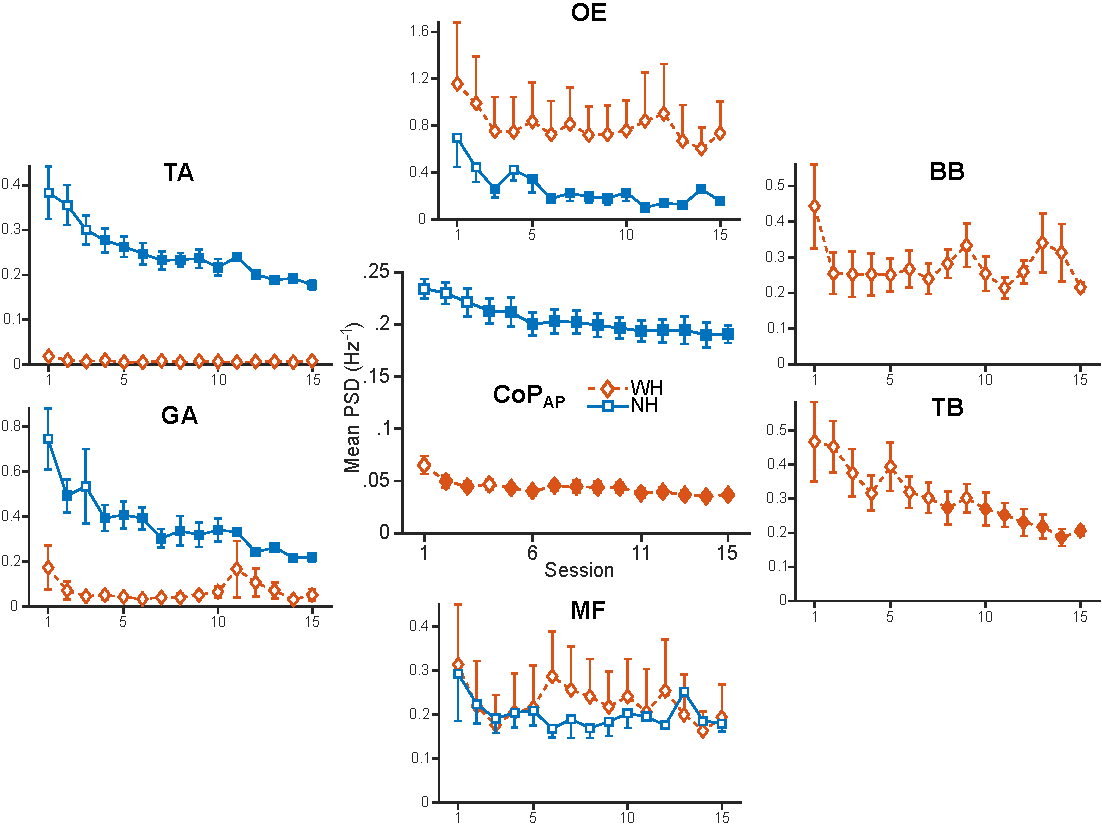
\includegraphics[width=\textwidth]{meanErrorBarsAll.pdf}
		\caption{Figure shows the effect of repeated sessions on muscle activation and CoP$_{AP}$ movement. Blue squares with SEM represent mean PSD in no handle and orange diamonds with SEM represent mean PSD in handle condition. Coloured markers indicate statistically significant sessions (mean values of individual session compared to the mean of the 1st session).}
		\label{fig:meanErrorBars}
	\end{center}
\end{figure}

We performed an analysis of differences in EMG activation levels between the two experimental stages in the frequency spectrum of the perturbation waveform (low = 0.25 - 0.5 Hz, medium = 0.5 - 0.75 Hz, high = 0.75 - 1.0 Hz). A paired samples analysis between the two stage for low, medium and high frequency range revealed that there was an influence of additional hand contact on both lower leg muscles. There were confirmed statistically significant differences between the two stages in all frequency ranges and for all sessions. For the MF muscle these differences were not significant in any of the frequency range nor session. However, there were significant differences between the two stages for the OE muscle. These differences occurred in the medium and high frequency range but only in the last session.

When the subjects were holding to the handle, we recorded the forces exerted on the handle during the continuous postural perturbations. Statistical analysis of handle forces revealed that the repetition of sessions had no significant effects (see Fig. \ref{fig:HandleForces}). Even though the activation of arm extensor muscle changed (decreased) during sessions, there was no significant change in forces applied on the handle.

\begin{figure}[!t]
	\begin{center}
		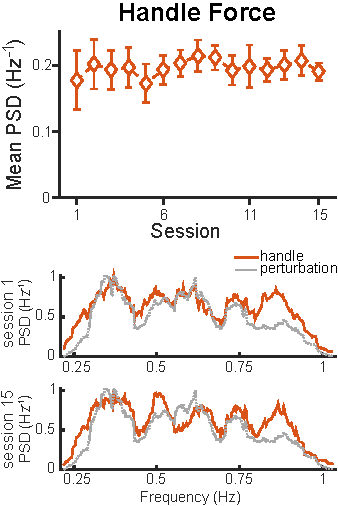
\includegraphics[width=0.5\textwidth]{HandleForce-all.pdf}
		\caption{The picture shows the handle force as recorded during the proposed experiments (see text).}
		\label{fig:HandleForces}
	\end{center}
\end{figure}


\begin{figure}
\centering
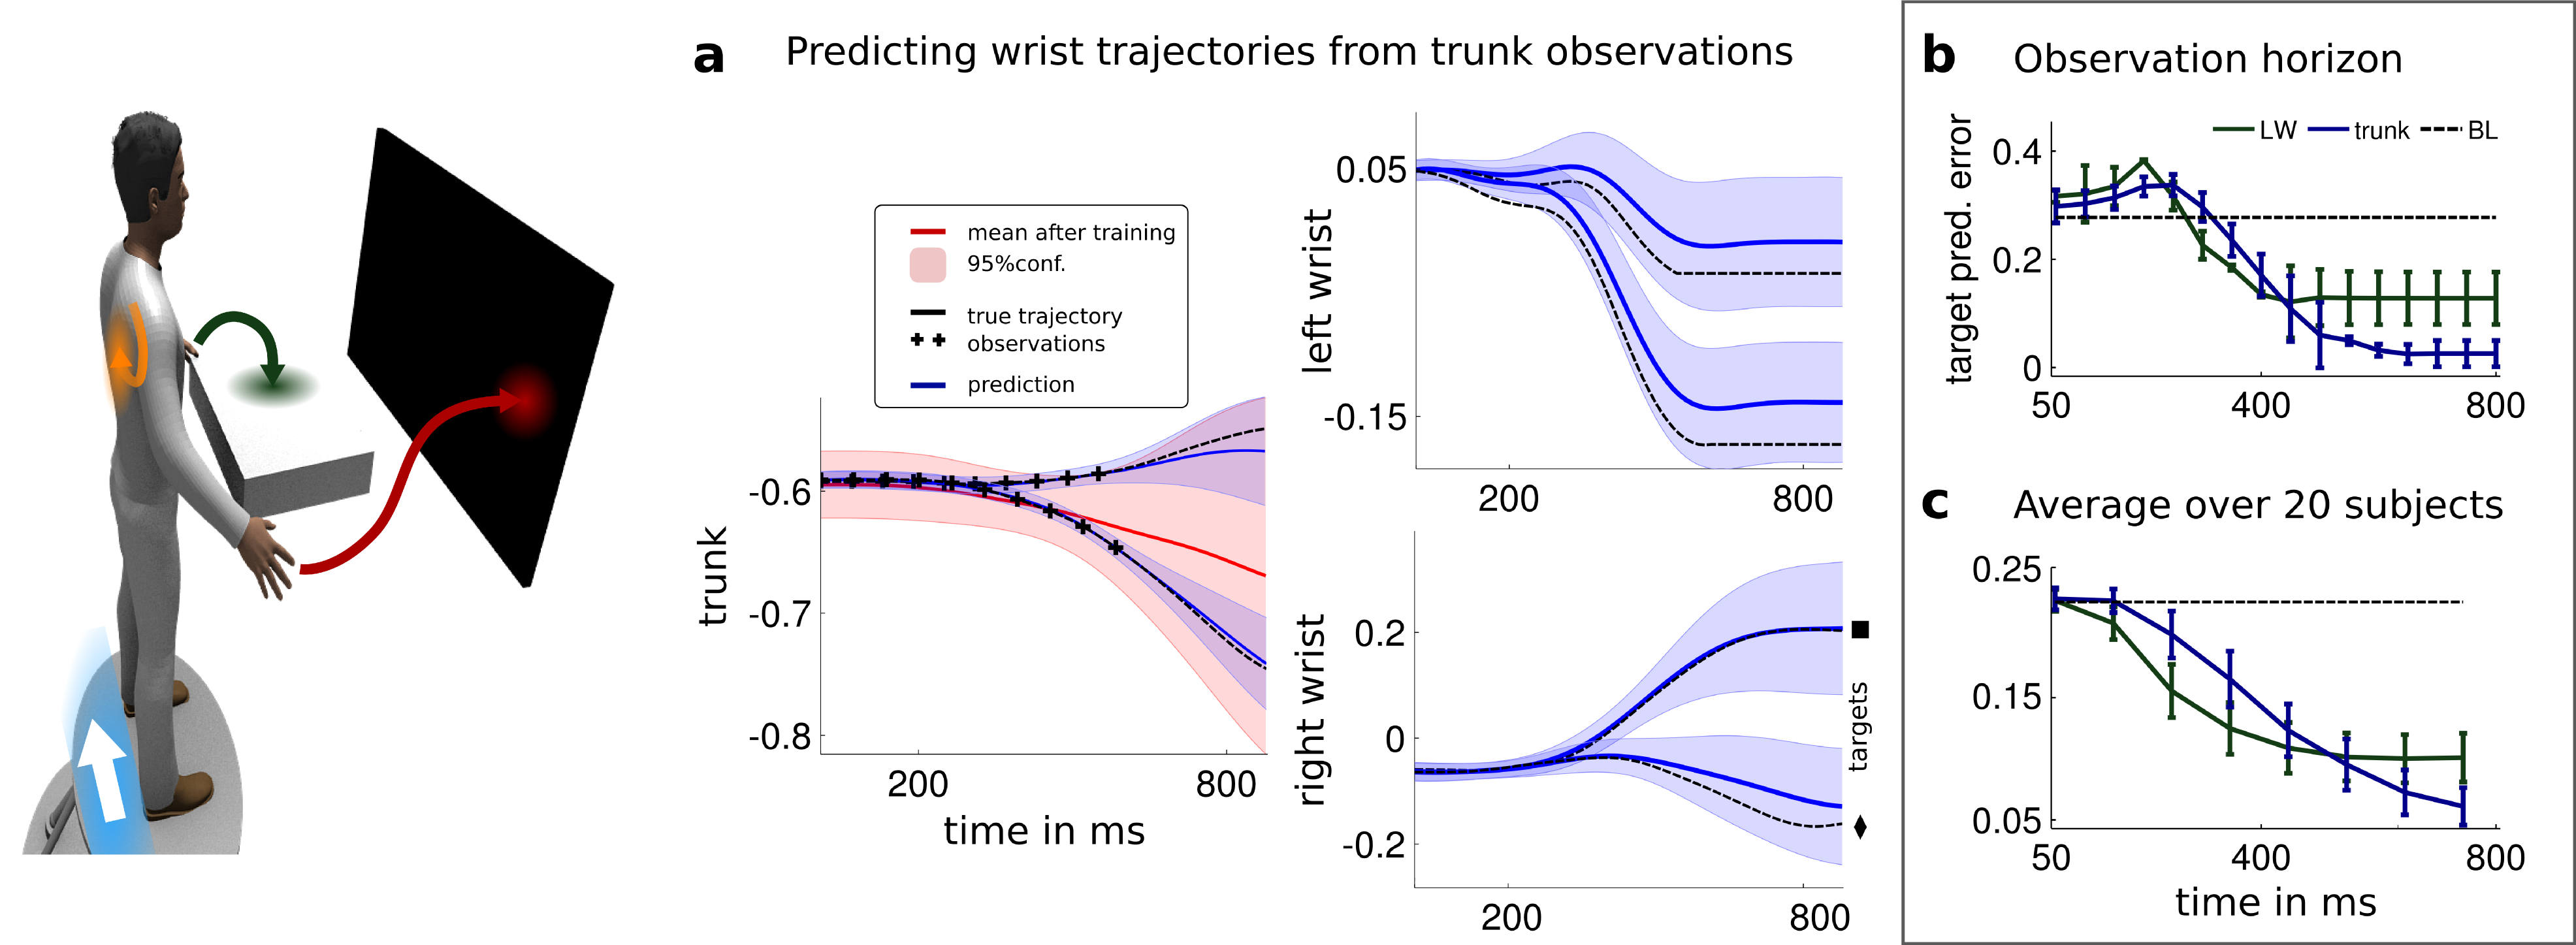
\includegraphics[width=0.8\textwidth]{SummaryFig_Y2Report.png}
\caption{Trunk trajectories predict wrist trajectories. (a) 600ms of trunk trajectories are observed. These observations can predict the wrist trajectories. Shown are predictions for the two exterior targets on the screen. For training 10 trials for each target are used starting from trial 240 backwards in time (before the catch trials). For testing the first perturbed trial after trial number 240 were used. (b) The effect of the observation horizon on the target prediction error is shown for a representative subject. The mean of the training data denotes the base line (BL). (c) Average statistics (mean and 95 percent confidence bound) over 20 subjects.
}
\label{fig:HumanProMPsPrediction}
\end{figure}

In collaboration with JSI, TUD studied whether supporting contacts in human arm reaching tasks are planned or an effect of a reactive controller. Investigations on human motor learning has focused on adaptation experiments with fixed contact points leaving research on the computational role of contacts as a free control variable unexplored.

In perturbed target reaching experiments sketched in Figure \ref{fig:HumanProMPsPrediction}, we studied weather supporting contacts are planned or reactive. Subjects had to reach for distant targets on a screen with their right hand. For reaching the target additional support through contacts with a table using the left hand was inevitably. If the contacts are planned then the left hand's motion can predict the right hand reaching.

We studied how probabilistic inference in learnt models can be used to answer this question. Evidence for planned contacts could be provided through learning probabilistic models of trajectory distributions and using the models to generate predictions, Figure \ref{fig:HumanProMPsPrediction} (a). We found that the target on the screen could be predicted from both, the left hand (mse: $10.4$cm $\pm$ $2$cm over $20$ subjects) and the trunk movement (mse: $6.7$cm $\pm$ $1.4$cm over $20$ subjects), which is illustrated in Figure \ref{fig:HumanProMPsPrediction} (b-c). The learnt probabilistic model could also be used to analyse the rate of adaptation of the left hand and the trunk kinematics, where the trunk trajectories converged faster than the left hand motion. This is intuitively explained by the strong need for corrective trunk movements in balancing. A report on the findings is currently in progress of writing.

Driven by the question on how human CNS optimizes arm reaching motions when the supportive hand contact has to be reached in order to maintain postural balance, UPMC and JSI started a combined experimental and computational study where the aim is to challenge two well-established but conceptually separated motor control phenomena: (i) Humans tend to reach faster to a target that looks more rewarding, despite the additional muscular cost of a faster movement \cite{Fitts1954}, and (ii) when humans have to be precise, movements take longer to perform \cite{Shadmehr2010}. The aim of our study is to experimentally disclose both phenomena and evaluate a novel computational model designed to join them. We obtained several very promising preliminary results indicating a general mechanism that can unify both phenomena and point out a global trade-off arising from the interactions between movement time, cost and accuracy. The experimental setup is shown in Figure ref{fig:UnifyingTwoPhenomena} A report on the findings is currently in progress of writing.


\begin{figure}
\centering
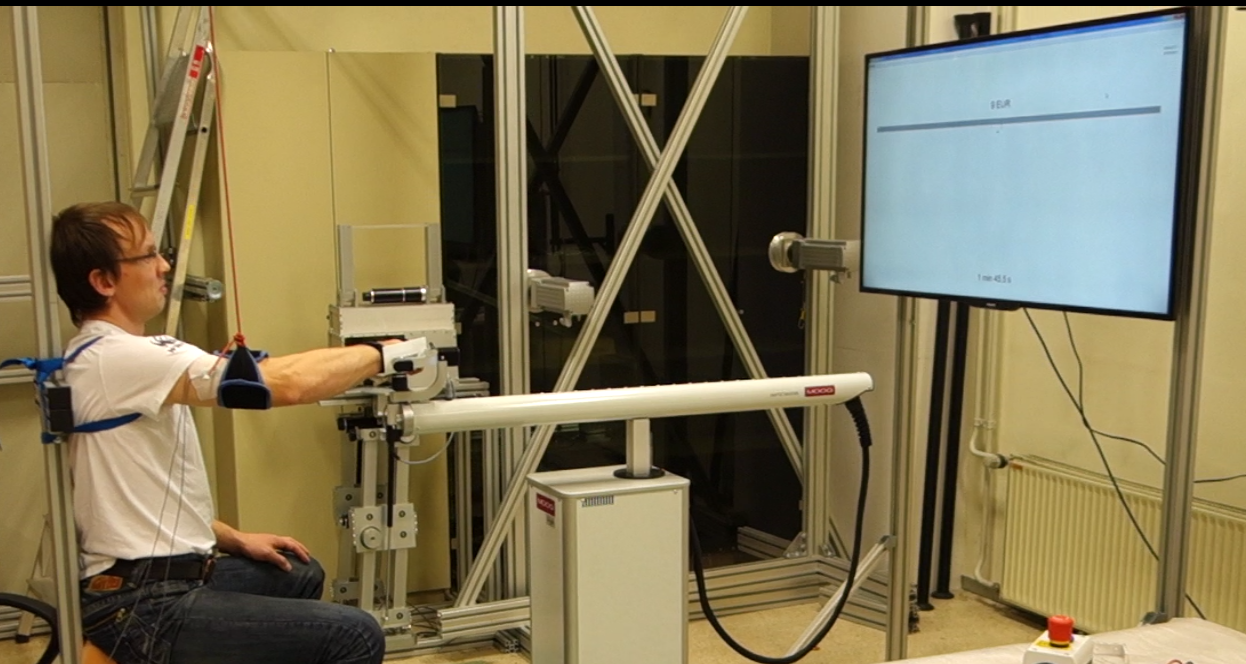
\includegraphics[width=0.8\textwidth]{UnifyingTwoPhenomena.png}
\caption{Experimental setup to understand how humans optimize arm reaching motions when the supportive hand contact has to be reached in order to maintain postural balance. The task of the subject was to obtain as high reward as possible in the given time by hitting a target on the virtual wall without knowing its actual size. In effect, the subjects had to find the optimal balance between precision, speed of motion and its cost in order to maximise the reward. To amplify the effect of cost of motion, haptic robot emulated a viscous media through which the subject had to move the hand.
}
\label{fig:UnifyingTwoPhenomena}
\end{figure}




